\documentclass{article}

\usepackage{arxiv}

\usepackage[utf8]{inputenc} % allow utf-8 input
\usepackage[T1]{fontenc}    % use 8-bit T1 fonts
\usepackage{hyperref}       % hyperlinks
\usepackage{url}            % simple URL typesetting
\usepackage{booktabs}       % professional-quality tables
\usepackage{amsfonts}       % blackboard math symbols
\usepackage{nicefrac}       % compact symbols for 1/2, etc.
\usepackage{microtype}      % microtypography
\usepackage{cleveref}       % smart cross-referencing
\usepackage{lipsum}         % Can be removed after putting your text content
\usepackage{graphicx}
\usepackage{natbib}
\usepackage{doi}
\usepackage[portuguese]{babel}
\usepackage{caption}


\graphicspath{ {../images/} }

\title{Quantum Oracles - Como transformar problemas clássicos em quânticos}

\date{}


\author{ \href{https://orcid.org/0009-0008-9134-5974}{
\includegraphics[scale=0.06]{orcid.pdf}\hspace{1mm}Alexandre Silva}\\
	Ciências da Computação\\
	UNIVEM - Centro Universitário Eurípides de Marília\\
}



\renewcommand{\headeright}{}
\renewcommand{\undertitle}{}
\renewcommand{\shorttitle}{}


\hypersetup{
pdftitle={Quantum Oracles - Como transformar problemas classicos em quanticos},
pdfsubject={quantum computing, computer science, ciencias da computacao, computacao quantica, algoritmos, algorithms},
pdfauthor={Alexandre Silva},
pdfkeywords={quantum oracles, quantum, quantum computing, algoritmos, algorithms},
}

\begin{document}
\maketitle

\begin{abstract}
	
\end{abstract}


\section{Introdução}
Hoje, não é díficil ver alguém falando sobre computação quântica e como essas máquinas vão mudar o futuro. Contudo, muitas dessas frases acabam se levando por extrapolações e/ou usos indevidos de ficção. Neste artigo, mostrarei que nem tudo é possível ser feito com um computador quântico atual, assim como existem pequenas áreas que se beneficiam ao máximo dessa nova tecnologia.\\
Para esse feito, serão mostrado alguns testes feitos usando o \href{https://www.ibm.com/quantum/qiskit}{qiskit}, um framework open source da IBM para computação quântica, além de alguns resultados obtidos após executar os algoritmos em simuladores e máquinas reais, assim como seus relativos em computação clássica. Algoritmos dos quais tomam proveito dos quantum oracles, modelos ideias de função que não ajudam a descrever o algoritmo matematicamente, também tomam proveito de alguns efeitos quânticos, como superposição e interferência, para se sobressair à algumas estratégias clássicas.\\
Com isso, o projeto foi desenvolvido em cima de cinco pequenos problemas, sendo eles: conversão de milhas para quilômetros, torre de Hanoi, explorador de arquivos, Buckshot Roulette e QRAM. Todas as implementações e materiais utilizados podem ser encontrados \href{https://github.com/Dpbm/scientific-initiation-1-quantum-oracles}{nesse repositório do GitHub}.


\section{Início do projeto}
Para dar início a pesquisa, foi necessário entender quais os tipos de oracles existem e como eles podem ser usados.\\
Em computação clássica, temos as Oracle Machines, as quais são maquinas de Turing, das quais implementam alguma função em seu interior, e ao ser chamado/invocado o resultado correto é retornado em tempo constante $O(1)$, podendo ser vista como uma caixa preta, abstraindo completamente o seu funcionamento. Devido a essa definição, as OMs são ideias matemáticos, sendo assim usados apenas para formalismo matemático.\\
Contudo em computação quântica, podemos de fato implementar certos modelos de Oracles e adiciona-los a um circuito maior, executando certas funções como: encoding de dados, aplicação de $f(x)$, abstração de partes do circuito, etc.

\subsection{Tipos de Oracles}

\subsubsection{Phase Oracle}
Um dos primeiros tipos de Oracles usados para a criação de algoritmos como os de: \href{https://en.wikipedia.org/wiki/Grover%27s_algorithm}{Grover} e \href{https://en.wikipedia.org/wiki/Deutsch%E2%80%93Jozsa_algorithm}{Deutsch–Jozsa}; é comummente conhecido como \emph{Phase Oracle}.\\
Tal dispositivo, é usado para atribuir uma fase ao circuito, sendo muito usado para configurar valores ou explorar a interferência.

\begin{center}
	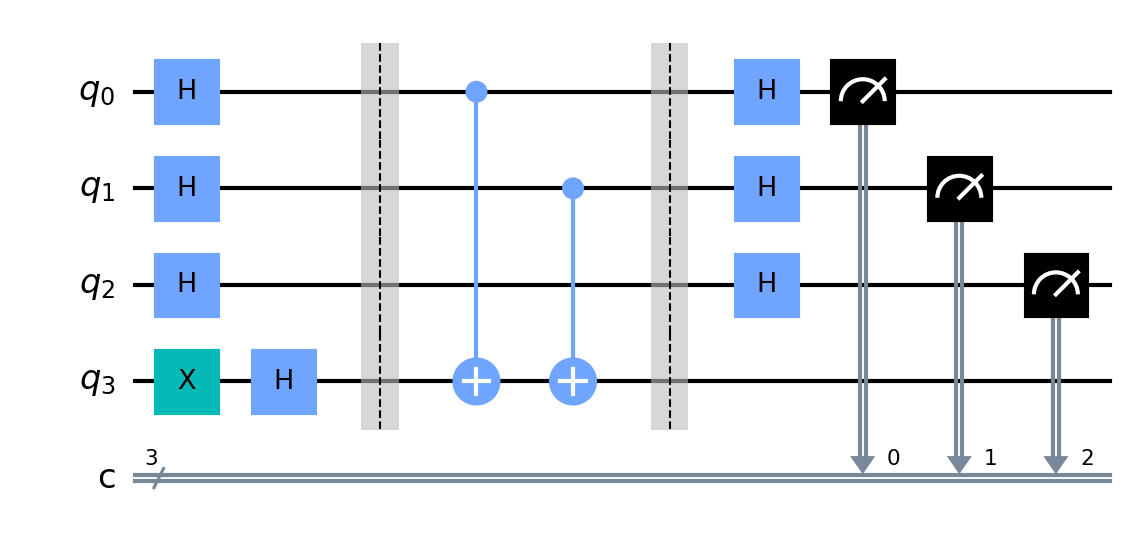
\includegraphics[scale=0.3]{phase_oracle_1.png}
	\captionof{figure}{Exemplo de phase oracle usado para o algoritmo de Deutsch–Jozsa}
	\label{fig:phase-oracle-1}
\end{center}





\section{Examples of citations, figures, tables, references}

\subsection{Citations}

\begin{center}
\end{center}


\bibliographystyle{unsrtnat}
\bibliography{references}  


\end{document}
